% manuscript, to be drafted

%%This is a very basic article template.
%%There is just one section and two subsections.
%\documentclass[12pt,oneside,a4paper,doublespacing]{article} % for submission
\documentclass[11pt,oneside,a4paper]{article} % for sharing

\usepackage{xfrac}
\usepackage{appendix}
\usepackage{amsmath}
\usepackage{caption}
\usepackage{placeins}
\usepackage{graphicx}
\usepackage{subcaption}
%\usepackage{subfig}
\usepackage{longtable}
\usepackage{setspace}
%\usepackage{tikz}
\usepackage{booktabs}
\usepackage{tabularx}
\usepackage{xcolor,colortbl}
\usepackage{chngpage}
%\usepackage[active,tightpage]{preview}
\usepackage{natbib}
\bibpunct{(}{)}{,}{a}{}{;} 
\usepackage{url}
\usepackage{nth}
\usepackage{authblk}
\usepackage[most]{tcolorbox}
%\usepackage{hyperref}
%\usepackage{color}
%\usepackage{fontspec}
%\usepackage{pdfsync}
\usepackage[normalem]{ulem}
\usepackage{amsfonts}
%\renewcommand{\listtablename}{List of Appendix Tables}
%\newcolumntype{C}[1]{>{\centering\let\newline\\\arraybackslash\hspace{0pt}}m{#1}}
%\newcolumntype{L}[1]{>{\raggedright\let\newline\\\arraybackslash\hspace{0pt}}m{#1}}
% working on this need to concatenate file name based on sex and variable name
%\newcommand\Cell[1]{{\raisebox{-0.05in}{\includegraphics[height=.2in,width=.2in]{Figures/ColorCodes/\expandafter#1}}}}  

%%%%%%%%%%%%%%%%%%%%%%%%%%%%%%%%%%%%%%%%%%%%%%%%%%%%%%%%%%%%%%%%%%%%%%%%%%%%%
% setting color to letters affects spacing. Here's a hack I found here:
% http://tex.stackexchange.com/questions/212736/change-letter-colour-without-losing-letter-spacing
%\DeclareRobustCommand{\spacedallcaps}[1]{\MakeUppercase{\textsc{#1}}} % all
% caps with better spacing

%\colorlet{RED}{red}
%\colorlet{BLUE}{b}
%\colorlet{rd}{red}
%\colorlet{bl}{blue}

%%%%%%%%%%%%%%%%%%%%%%%%%%%%%%%%%%%%%%%%%%%%%%%%%%%%%%%%%%%%%%%%%%%%%%%%%%%%%%

\newcommand\ackn[1]{%
  \begingroup
  \renewcommand\thefootnote{}\footnote{#1}%
  \addtocounter{footnote}{-1}%
  \endgroup
}
%\newcommand\vt[1]{\textcolor{rd}{#1}}
%\newcommand\eg[1]{\textcolor{bl}{#1}}

%\newcommand\tg[1]{\includegraphics[scale=.5]{Figures/triadtable/triad#1.pdf}}
%\newcommand\tgh[1]{\raisebox{-.25\height}{\includegraphics[scale=.3]{Figures/triadtable/triad#1.pdf}}}

\defcitealias{HMD}{HMD}
\newcommand{\dd}{\; \mathrm{d}}
\newcommand{\tc}{\quad\quad\text{,}}
\newcommand{\tp}{\quad\quad\text{.}}
% junk for longtable caption
\AtBeginEnvironment{longtable}{\linespread{1}\selectfont}
\setlength{\LTcapwidth}{\linewidth}

%%%%%%%%%%%%%%%%%%%%%%%%%%%%%%%
\begin{document}

\title{Accounting for temporal variation in morbidity measurement
and projections}

\author[1]{Alyson van Raalte\thanks{vanraalte@demogr.mpg.de}}
\author[1]{Tim Riffe}
%\author[3]{John MacInnes}
\affil[1]{Max Planck Institute for Demographic Research}
%\affil[2]{Department of Demography, University of California, Berkeley}
%\affil[3]{School of Social and Political Science, University of Edinburgh}

%\author{[Authors]}

\maketitle

\begin{abstract}
This is important stuff!
\end{abstract}

$G$ is a bad health condition that varies as a function of time to death,
$y$ and not as a function of chronological age, $a$. However, there will still be an
apparent age function, $g'(a)$, given that $g(y)$ is regular and mortality is
sort of stable, but not really. $g'(a)$, in this case, is an aggregate based on
both mortality and the real underlying time-to-death process:
\begin{align}
g'(a) &= \frac{\int _0^\omega g(y) N(a,y) \dd y}{N(a)} \\
      &= \frac{\int _0^\omega g(y) N(a)
      \mu(a+y)\frac{\ell(a+y)}{\ell(a)}\dd y}{N(a)}\\
      &= \int _0^\omega g(y) f(y|a)\dd y
\end{align}
a little excercise we still need to do: find the $g'(a)$ that belongs to $g(y)$
in our canned example. It will be different for males and females because they
have different mortality schedules. In this case, we can make the healthy l;ife
expectancy function be based on mortality and $g'(a)$ and see what would be the
prediction if $g'(a)$ is held constant and we induce mortality improvement. The
answer is that mortality improvement will appear to increase the proportion of
remaining life expectancy that is unhealthy: also the absolute years spent
unhealthy, but the change in sex gap is maybe ambiguous (gotta check, maybe
not), depending on the changes induced.


brief interlude \ldots.
This is a simple caes of $g(y)$, but in reality morbidity often varies as a
function of both chronological and thanatological age, and we ought to have a
function $g(a,y)$.

\section{temp section, out of sync, just for latex}

Given the numbers from Figures X, there are various methods that one can use to
calculate period and cohort lifetables. For the sake of reproducibility for our
toy example, we describe steps as follows, firs tfor periods, then for cohorts.
\subsection{Period quantities}
We use event exposure lifetables, though it would be possible to jump straight
to death quotients from the given Lexis diagram.
Exposures for age $x$ in year $t$, $E(x,t)$, are calculated, per the HMD Methods
Protocol (cite) as:
\begin{equation}
E(x,t) = \frac{C(x,t) + C(x,t+1)}{2} + {D_L(x,t) - D_U(x,t)}{6} \tc
\end{equation}
where $C(x,t)$ is the census population in age interval $[x,x+1)]$ on January 1
of year $t$, $D_L(x,t)$ are deaths in the lower Lexis triangle of age $x$ in
year $t$, i.e., belonging to the cohort born in the year interval $[t-x,t-x+1)$.
$D_U(x,t)$ are deaths in the upper Lexis triangle of age $x$ in
year $t$, i.e., belonging to the cohort born in the year interval
$[t-x-1,t-x)$. All standard period lifetable steps are followed from the HMD
Methods Protocol, with the exception of the $a(x)$ assumption. The HMD assumes period $a(x)$
values of $\frac{1}{2}$. Instead, we apply the following formula:
\begin{equation}
a(x,t) = \frac{D_L(x,t)\frac{1}{3} + D_U(x,t)\frac{2}{3}}{D_L(x,t) + D_U(x,t)}
\tp
\end{equation}
We then proceed to calculate all columns through $e(x)$. 

The average value of the unhealthy condition $G$ at age $x$in year $t$, $g(x,t)$
is calculated as follows. We first convert counts unhealthy on birthdays to
proportions, and then take the arithmetic average of the proportion unhealthy at
age $x$ and age $x+1$. Expectancies are then calculated as follows:
\begin{align}
e(0,t) =&\sum _0^2 L(x,t) \\
e_U(0,t) =&\sum _0^2 L(x,t) g(x,t) \\
e_H(0,t) =& e(0,t) - e_U(0,t) \tc
\end{align}
where $e(0,t)$ is the life expectancy at birth in year $t$, $e_U(0,t)$ is
unhealthy life expectancy, and $e_H(0,t)$ is healthy life expectancy.

\subsection{Cohort quantities}
For cohorts we procede directly from within-cohort age interval survival
probabilities, $p(x,c)$, as follows:
\begin{equation}
p(x,c) = \frac{B(x+1,c)}{B(x,c)} \tc
\end{equation}
where $B$ are birthdays (horizontal counts), $x$ indexes the lower age interval
bound, and $c$ is the cohort born in the year interval $[c,c+1)]$. Starting with
a radix of 1, we calculate $l(x,c)$ as:
\begin{equation}
l(x,c) = \prod_0^x p(a,c)
\end{equation}
$L(x,c)$ is calculated as the arithmetic average of lower $l(x,c)$ and
$l(x+1,c)$. The average value of $G$ for the AC parallelogram is calculated
similarly as for period squares, except that we take the arithmetic average of
the proportions unhealthy at birthday $x$ and $x+a$ within the same cohort.
Expectancies are then calculated in the same way.

\subsection{Values assumed for $g(y)$ in toy example}
If deaths in Lexis triangles are distributed uniformly, then the average year
lived of those dying in the triangle is $\sfrac{1}{3}$. Since deaths in the
example Lexis diagram are given in triangles, we assume values of $g(y)$ for the
average years lived for the deaths in each triangle. For example, 20 of the
babies born in the year 2003 will die within the year, and these have an average
lifespan of $\sfrac{1}{3}$, and so they contribute $20\times0.90$ unhealthy
people to the birth cohort at age 0. 

 \begin{table}[ht]
\centering
\begin{tabular}{rr}
\hline
TTD & $g(y)$ \\
\hline
$\sfrac{1}{3}$ & 0.90 \\
$\sfrac{2}{3}$ & 0.60 \\
$1\sfrac{1}{3}$ & 0.20 \\
$1\sfrac{2}{3}$ & 0.10 \\
$2\sfrac{1}{3}$ & 0.05 \\
$2\sfrac{2}{3}$ & 0.02 \\
\hline
\end{tabular}
\caption{$g(y)$ used in toy example.}
\label{tab:gy}
\end{table}

\section{Morbidity as a function of thanatological age}
 
Imagine a bad health condition, $G$, that varies as a function of time to death,
$y$, and not as a function of chronological age, $a$. Since the distribution of
times to death is empirically regular, there will still be an apparent age
function, $g^\star(a)$.
In this case $g^\star(a)$ is an aggregate based on both mortality and the real underlying time-to-death process:
 
\begin{align}
g^\star(a) &= \frac{\int _0^\omega g(y) N(a,y) \dd y}{N(a)} \\
      &= \frac{\int _0^\omega g(y) N(a)
      \mu(a+y)\frac{\ell(a+y)}{\ell(a)}\dd y}{N(a)}\\
      &= \int _0^\omega g(y) f(y|a)\dd y \tc
\end{align}
where $N(a)$ is the population aged $a$, $\ell(a)$ is the survival function, and
$\mu(a)$ is the force of mortality. $f(y|a)$ can be interpreted as the
probability of dying in $y$ years given survival to age $a$, and thus the final
expression is purged of population structure. That is, the population of age $a$
that has condition $G$ does not depend on population structure at all, but only
on the force of mortality and the time-to-death pattern of $G$, $g(y)$. 

A function such as $g(y)$ would have implications for the interpretation of
period age patterns of morbidity, and by extension, healthy life expectancy
(HLE). If a function such as $g(y)$ holds, it is tautologically true that the
measurement of HLE in completed cohorts (or populations with fixed mortality)
will be identical whether estimated on the basis of $g^\star(a)$ or $g(y)$.
Period HLE is also unproblematic in a fixed mortality setting, as long as future
mortality is also held fixed. Difficulties only arise in the interpretation of
period HLE under changing mortality. For a time-to-death process, forthcoming
improvements in mortality will have the effect of decreasing morbidity today.
This artifact can stymie the projection of today's age patterns of morbidity
into the future: Under changing mortality and a fixed $g(y)$, the age pattern of
morbidity will change even as the morbidity process does not. 

Further, since morbidity is partly a function of mortality, it is difficult to
compare the age patterns of morbidity for populations with different mortality
levels or patterns. Under these circumstance, it is trickier than it seems to
partition differences period HLE into true morbidity and mortality components, because the morbidity component will rely on some unknown future mortality quantity that is a driver of the apparent age pattern of morbidity.
 
We first illustrate this concept with a toy example. Assume the population
process outlined in the Lexis diagram of Figure~\ref{fig:Fig_DiagramLexis}. This
diagram represents quantities that will induce the aforementioned inconsistency.
Blue numbers on the horizontal age bars represent the number of birthdays, while
black numbers represent cesnsus counts. Red numbers represent deaths in the
Lexis triangle, and finally, green numbers next to birthdays represent the
number of unhealthy people that would be alive assuming the pattern of $g(y)$
found in Figure~\ref{fig:Fig_TTDgy} (given in Appendix Table~\ref{tab:gy}) and
the given mortality pattern, assuming deaths are distributed uniformly in Lexis
triangles, and the average values given in Table~\ref{tab:gy} apply. The example
moves from a higher mortality stationary setting to a lower mortality stationary
setting.

\begin{figure}
\begin{adjustwidth}{-1.5cm}{}
	\centering
	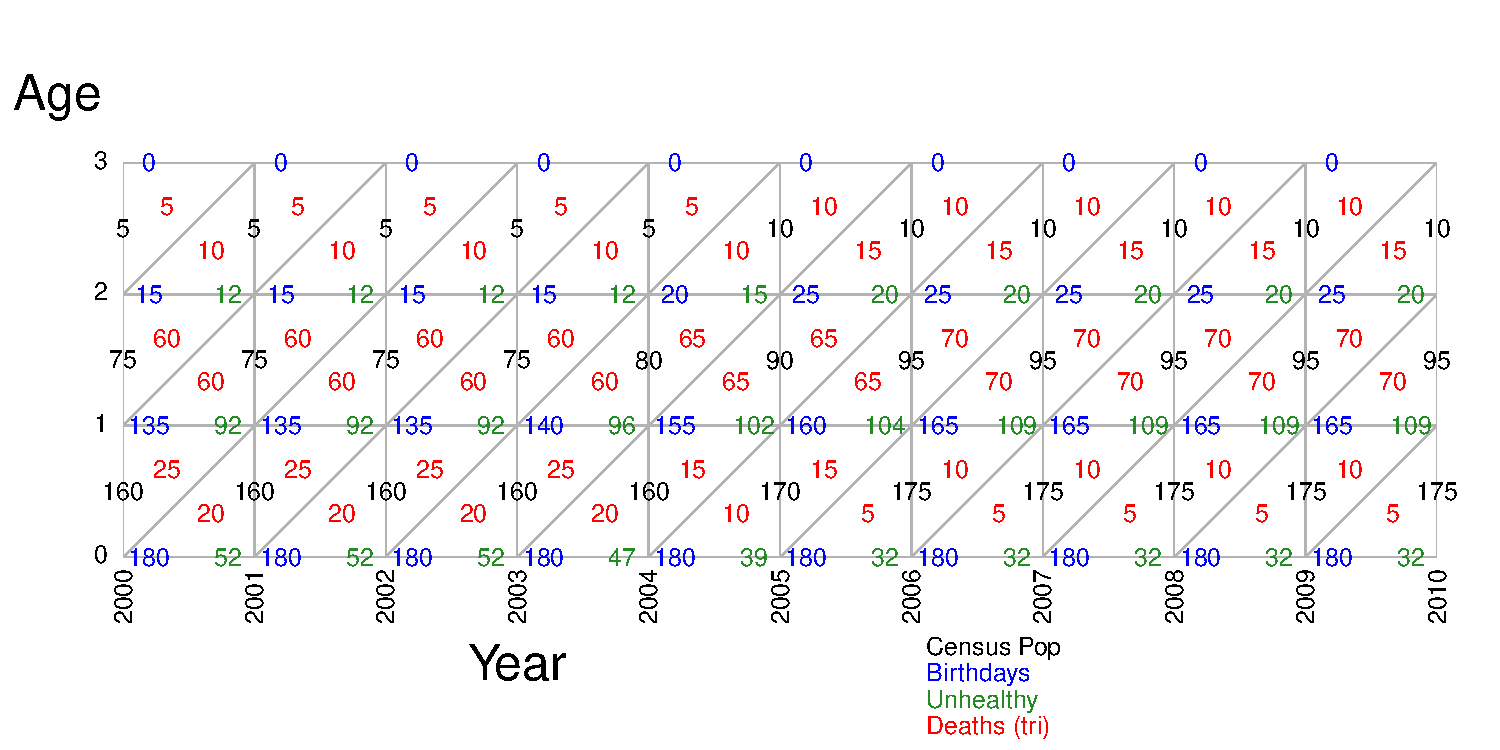
\includegraphics[scale=.6]{Figures/DiagramLexis.pdf}
	\caption{The Lexis diagram}
	\label{fig:Fig_DiagramLexis}
\end{adjustwidth}
\end{figure}

\begin{figure}
\begin{adjustwidth}{-1.5cm}{}
	\centering
	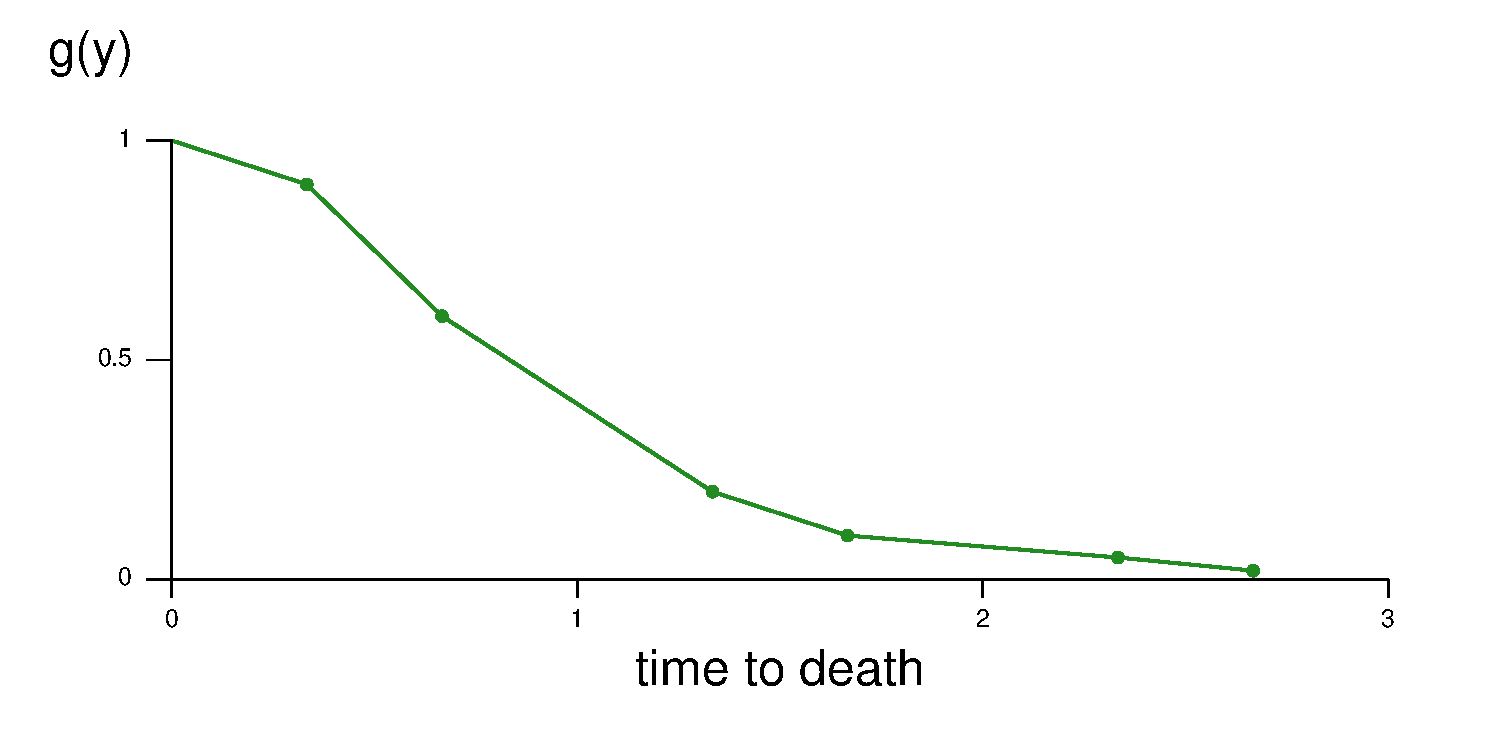
\includegraphics[scale=.6]{Figures/TTDgy.pdf}
	\caption{The time-to-death profile of disability}
	\label{fig:Fig_TTDgy}
\end{adjustwidth}
\end{figure}

To calculate the numbers unhealthy in any given birthday line, first note that
the average years lived in a Lexis triangle by those dying in the triangle is
$\sfrac{1}{3}$. For example, 20 of the
babies born in the year 2003 will die within the year. These deaths have an
average lifespan of $\sfrac{1}{3}$, and so they contribute $20\times0.90$ unhealthy
people to the birth cohort at age 0 (value from appendix table~\ref{tab:gy}.
Those dying from the same cohort before age 1 in the year 2004 contribute
$15\times0.6$ unhealthy persons to age 0 in 2003, and so forth iteratively up
the cohort.

In this controlled setting, where the underlying $g(y)$ is held fixed, we can
calculate both the period and cohort HLE values.\footnote{See Appendix
explanations for the details used to calculate lifetables and mean values of
$G(a)$. } Figure~\ref{fig:e0eHtoy} shows trends in period and cohort total and
healthy life expectancy. In the initial and final stages, period and cohort
healthy and total life expectancies agree, because these are the stationary
start and end of the series. As is usually the case, there is no perfect way to
compare cohort and period line graphs, since the x-axis refers to both cohort
and period. 

\begin{figure}
\begin{adjustwidth}{-1.5cm}{}
	\centering
	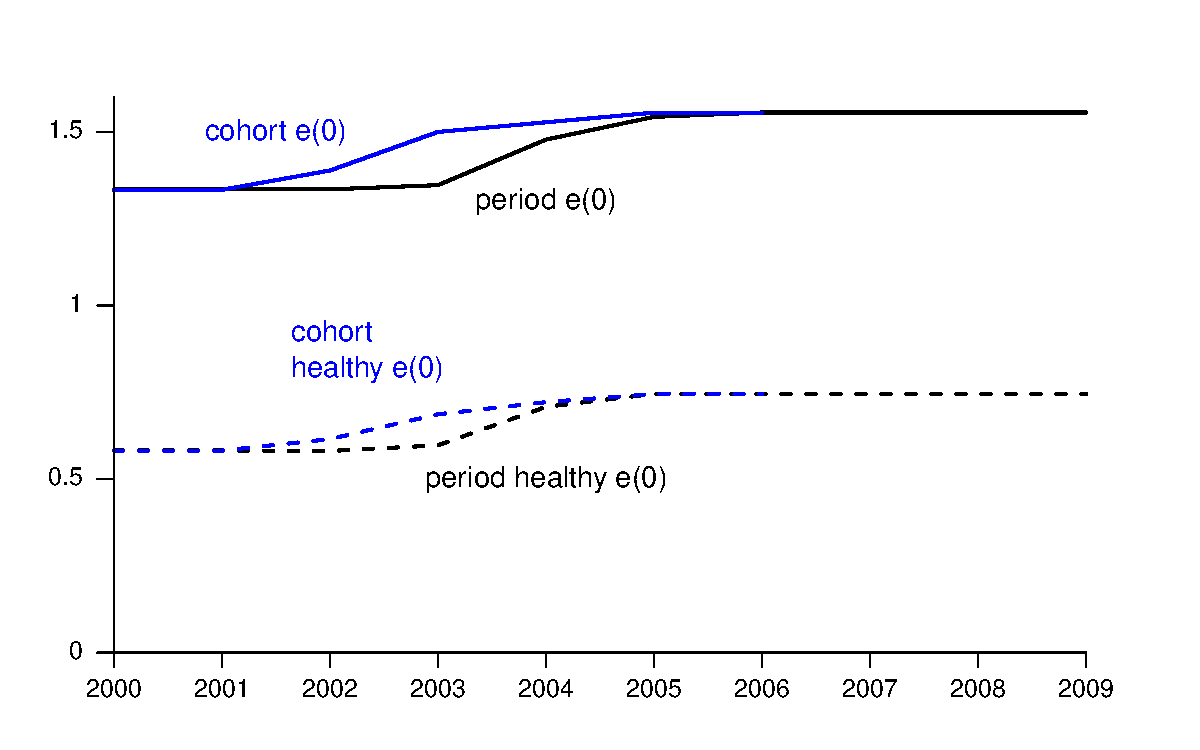
\includegraphics[scale=.6]{Figures/e0eHtoy.pdf}
	\caption{Cohort and period life expectancy and healthy life expectancy.}
	\label{fig:e0eHtoy}
\end{adjustwidth}
\end{figure}

The gap between year 2001 and 2005 marks an inconsistency. In
this case, the inconsistency is entirely driven by mortality change. Further the
gap in HLE is due not only to the change in the survival function used to
calculate HLE, but also to changes in the pattern of $g^\star(a)$. That is,
if we were to decompose the difference in 2001 and 2007 HLE using conventional
methods, there would appear to be a morbidity contribution to the difference,
even though morbidity in this case is held fixed. We demonstrate such an
inconsistency using somewhat more realistic data in a following section.
 
In reality, not all end-of-life health conditions are exclusive functions of
time-to-death, but morbidity often varies as a function of
both chronological and thanatological age, and it is best to express morbidity
as a function of both age and time-to-death, $g(a,y)$. There is great variety in
the temporal variation of late-life health conditions (cite Riffe 2015 MPIDR
working paper.) Further, the function $g(a,y)$ changes over time and it is not
fixed as in our example. The distortion demonstrated is however likely to arise
in everyday practice when comparing health trends over age between populations
and over time, since many health conditions appear to show strong time-to-death
componenents. Trends in mortality may offset or amplify changes in morbidity.
Therefore, in order to separate effects, more careful measurements are required
than is typically the case. We provide another expository example in a more
realistic setup.
 


















\end{document}